\section{Adjacent Ideas and Ecological Adoptions}

Ecological concepts have been adopted by many different disciplines over the course of the twentieth century (see figure 2). An examination of some of these adoptions helps illuminate the emergence of information ecology in the late 1990s. Three examples of ecological concepts migrating into other disciplines will be discussed: cognitive ecology, media ecology, and political ecology. Each of them shows how ecological concepts can be adopted by a discipline for many different purposes. Purposes which may be renegotiated at any time.

\begin{figure}[!ht]
  \centering
    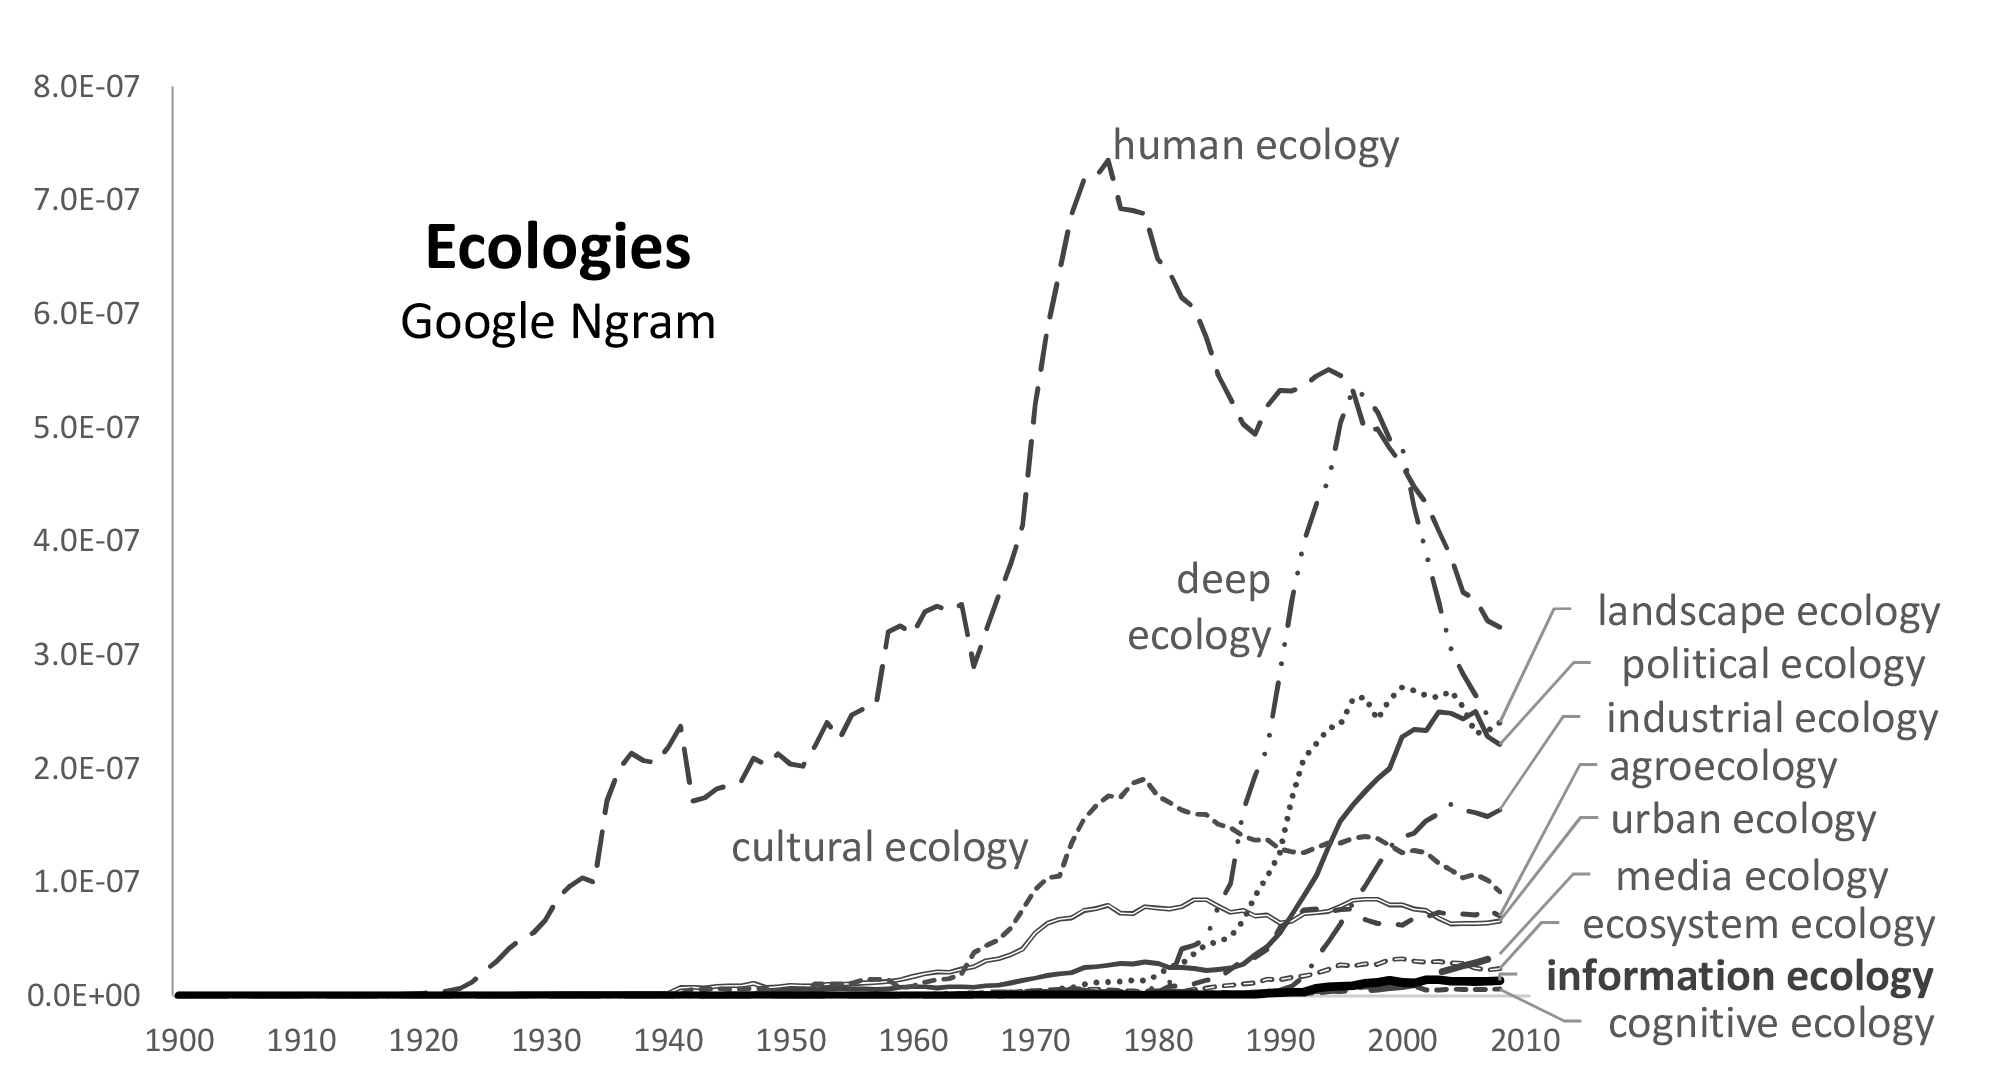
\includegraphics[width=5.5in]{figures/ecologiesAll}
  \caption{Emergent ecologies as a Google Ngram. Note the early dominance of human ecology and then deep ecology; only in the 1990s did ecological thinking become broadly adopted in many disciplines.}
\end{figure}

\subsection{Cognitive Ecology}

In a review of cognitive ecology Hutchins \citep{hutchins_cognitive_2010} discusses the sources of the field and how it interacts with cognitive science. He writes that "Cognitive ecology is the study of cognitive phenomena in context. Elements of cognitive ecology have been present in various corners, but not the core, of cognitive science since the birth of the field. It is now being rediscovered as cognitive science shifts from viewing cognition as a logical process to seeing it as a biological phenomenon" \citep[][p. 705]{hutchins_cognitive_2010}. 

Hutchins contrasts logical and biological approaches to understanding cognition; early cognitive science was faced with a tension between reductionism and holism. Two schools of thought, a cybernetic and an information processing approach, emerged from the early ferment of the field. Cyberneticists, such as Gregory Bateson, emphasized the interactions between mind and the environment. He wrote an influential book in 1972 titled \textit{Steps to an Ecology of Mind} as a theoretical manifesto for paying greater attention to the interconnections between environment and the mind \citep{bateson_1972}. On the other hand information processing advocates concentrated on the parallels between the digital computer and the mind. The focus on the digital computer reduced the activity of the mind to symbolic event processing, relegating perceptual systems and the motor systems used to interact with the world to the periphery of the field of cognitive science. Cognitive science is revising itself and reexamining the connections between the world and the mind through cognitive ecology \citep{hutchins_cognitive_2010}.

One of the emergent themes in cognitive ecology is this contrast between the digital and the biological. Cognitive science, as a field, chose to use a digital-technological paradigm [reductionist?] in order to manage the scope of its studies and to define the appropriate units of analysis for its research efforts. While critics of this approach were present from the beginning, their more hoistic and contextual approaches were often marginalized in post WWII funding circles. Context becomes one of the key concepts for both motivating and operationalizing a holistic shift in thinking, nevertheless. Motivating because context is key in a proper discussion of an information environment, and operationalizing because context points to the people and groups which surround and interact with any socio-technical system as a new unit of analysis.

Another emergent theme in cognitive ecology is mutual dependence. From the abstract of Hutchins review, cognitive ecology "points to the web of mutual dependence among elements of a cognitive ecosystem." \citep{hutchins_cognitive_2010}. In \textit{Cognition in the Wild} Hutchins described the process used to navigate large Navy ships, which are excellent examples of the mutual dependence between people, technology, and information. Each component of the system, or ecology [sic], needs to be functioning well in order to achieve the overall goal of determining the ship's position. Mutual dependence is also a principal feature within discourses about the value of biodiversity \citep{hutchins_1995}. This theme is later picked up within the business management literature on information ecology.

\subsection{Media Ecology}

Just as cognitive ecologists can trace back to original controversies over holism and reductionism, media ecologists can trace a similar debate in their own field of communication between qualitative and quantitative methods. Much of the early research in the field of communications tried to emulate the natural sciences and adopted quantitative methods from postwar social sciences. Early studies on propaganda and other communication topics adopted a simplistic view of information transmission, which was later derided as the hypodermic [what does this mean here?] or administrative model of communication. The scientistic view of communication would not be challenged until the 1960s and 1970s. Throughout this time there were researchers who approached media and communication studies from a critical point of view, including thinkers such as Marshall McLuhan, Walter Ong, and Neil Postman.

The network formed by McLuhan, Ong, and Postman is often cited as the foundation for media ecology studies. All three of these thinkers discussed the meaning of their own work and explicitly framed much of that work in environmental terms. Postman is usually credited with the earliest use of the term media ecology in a 1968 talk, later published in 1970. He defined media ecology as "the study of media as environments." \citep{strate_media_2004} McLuhan described the relationship between different types of media and how they effected the mental environment.

\begin{quote}
The medium is the message” means, in terms of the electronic age, that a totally new environment has been created. The “content” of this new environment is the old mechanized environment of the industrial age. The new environment reprocesses the old one as radically as TV is reprocessing the film. For the “content” of TV is the movie. TV is environmental and imperceptible, like all environments. We are aware only of the “content” or the old environment. When machine production was new, it gradually created an environment whose content was the old environment of agrarian life and the arts and crafts. This older environment was elevated to an art form by the new mechanical environment. The machine turned Nature into an art form. \citep{mcluhan_understanding_2013} (p. 13)
\end{quote}

Ong writes about the "ecological concern" he believed media ecology would address, especially because "Its thrust is the dialectical opposite of the isolating thrust of writing and print." He described how evolutionary thinking proposed by Darwin demonstrated the development of organisms over time through the interaction of individuals and the environment. "The new philosophical attention to openness appears not unrelated to the opening of previously isolated human groups to one another fostered by electronic communications media, telephone, radio,
and ultimately television" \citep[][p. 324]{ong_interfaces_1977}.

Turning toward the environment in which communication and media interacted suggested a way to broaden the analysis of media in order to develop a broader critique of media in society. A more contemporary definition of media ecology is

\begin{quote}
how the form and inherent biases of communication media help create the environment or symbolic and cognitive structure in which people symbolically construct the world they come to know and understand, as well as its social, economic, political, and cultural consequences. \citep{lum_introduction:_2000}
\end{quote}

After the 1970s the study of media ecology spread in multiple directions. Ong focused on the distinction between orality and literacy, Postman became an influential public intellectual and critic of television, and McLuhan became famous his quote that the "medium is the message." Intellectual groups coalesced around many of these figures, especially in Toronto and New York, where McLuhan and Postman respectively spent much of their careers. In 1998 the Media Ecology Association was established and solidified the use of the term media ecology. 

Two themes from media ecology are worth considering when examining the adoption of ecology into different disciplines. The first is the idea of the environment. McLuhan describes how technology has created a totally new environment in which people are now embedded. Moreover, the media and technology environment is often ignored or even imperceptible to the people who live inside of it. There is a historical evolution of communication technologies in which older environments are replaced by newer ones. The second theme is raised by Ong when he talks about the openness engendered by the work of Darwin. Before Darwin species were considered separately from their environment, afterwards the connections between individual and environment are paramount. Technology, in the form of electronic communication devices and networks, transforms human society in an analogous way, bringing together groups which were previously isolated.

\subsection{Political Ecology}

Political ecology emerged in Geography in the later decades of the 20th century. Credit for the first use of the term is generally given to Eric Wolf in his 1972 article discussing environmental management in the Swiss Alps and how ownership of and access to resources structure environmental outcomes \citep{wolf_1972}. Very generally "[t]he phrase 'political ecology' combines the concerns of ecology and a broadly defined political economy. Together this encompasses the constantly shifting dialectic between society and the land-based resources, and also within classes and groups within society itself." \citep[][p. 17]{blaikie_1987}. 

Often political ecology is defined not as a discipline but as an approach to understanding the degradation of socio-natural systems that puts historical, political and economic context at the forefront of any explanation. This approach provides an alternative to the standard development trope that population pressure begets degradation of the environment: poverty and environmental degradation are in a dialectical relationship that can spiral downwards if only one factor is considered in policy formation for development \citep{blaikie_1987, peet_1996}.

Political ecology also emerged as a critique of the small scale studies from earlier human ecology and cultural ecology, yet it retained the emphasis on the governance of, and access to, natural resources in the overall explanations of system dynamics. Social justice is framed as an issue of access to and control of natural resources through property rights, which then can be used as an explanatory factor for socio-natural outcomes. This approach leads to alternative explanations of the tragedy of the commons thesis. Instead of inevitable degradation of the common "pasture" in Hardin's example--notably drawn from his work with bacteria in a petri dish, not people in a society--resources owned under common property regimes and governed by local practice and custom are often sustainably managed. While reminiscent of earlier human ecology, these alternate political ecological explanations fully acknowledge the problems of scale, complexity and context \citep{ostrom_1999}. 

A secondary, yet similarly powerful, framing of political ecology is that of the politics of environmental science. This framing explicitly gives science, and the knowledge, information and raw data that science produces, political agency in the policy arena. Social justice is framed as an issue of the control of, access to and use of the scientific information \citep{forsyth_2003,leach_1996}. The work of Gregory Bateson was important in the development of political ecology conceived in this manner \citep{peet_1996}.

Both approaches provide alternative explanations to popular "success" stories of conquest and colonialism. Due to the explanatory power of guns, disease, and metallurgical technology as primary factors in the pro-colonial outcomes of the conquistadores in the New World \citep[cf.][]{diamond_1997}, attention to secondary factors is often overlooked. Political ecologists draw attention to non-primary factors, such as the conquistadors desire for power, wealth and recognition, and the role of access to and control of resources in reaching these goals. The "success" of the conquest was not a "natural" or "god-given" outcome depicted as geographical luck of the European conquistadores, but instead a bloody tale of savagery and pillage. 

Together these framings draw heavily upon the narratives of ecologist as manager and the ecologist as activist. This has been heavily criticized, nevertheless. On the one hand, the approach is accused of being apolitical and only maintaining a superficial engagement with the political science literature \citep{walker_2007}. On the other hand, political ecology receives criticism for not including enough ecological thought and leaving explanations of environmental degradation to only political and economic factors \citep{vayda_1999,walker_2005}. In a sense political ecology fits well with Holling's observation that holistic approaches tend to offer answers of limited use to real problems \citep{holling_1998}. At the same time political ecology provides an example for information ecology and how to embrace interdisciplinary attempts to solve "wicked problems" at planetary scales.

\subsection{Ecologies vs Ecosystems}

In the examples above ecosystem metaphors--the cognitive ecosystem, the media ecosystem, the political ecosystem, and so on--are less used than the referents to the various ecologies (see figure 3). Within the academy, the various ecologies use ecological approaches to answering research questions. This might mean using some tools from the ecology toolkit or even thinking broadly about the relationships between the living and the non-living. 

\begin{figure}[!ht]
  \centering
    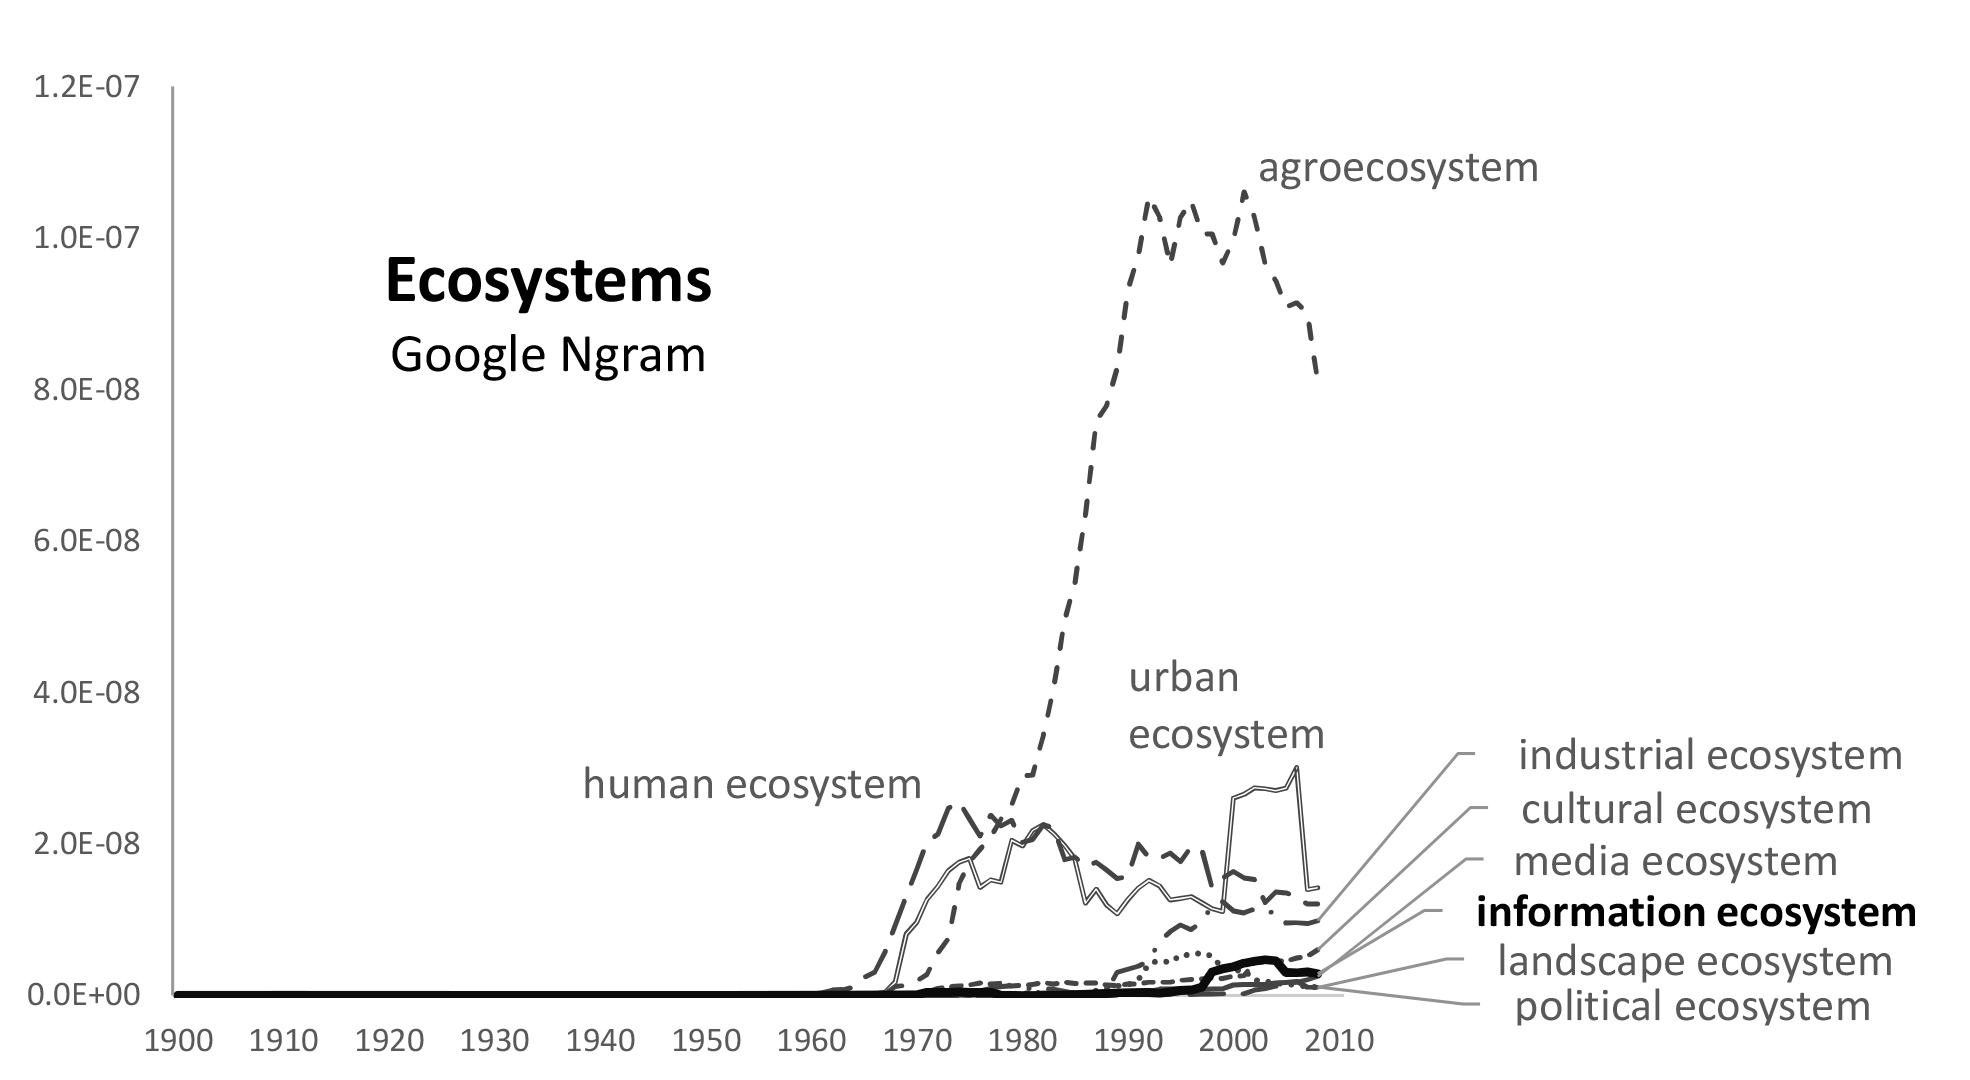
\includegraphics[width=5.5in]{figures/ecosystemsAll}
  \caption{Emergent use varying ecosystem metaphors as a Google Ngram. Compare to figure 2! The use of various ecologies vs various ecosystem metaphors is an order of magnitude higher.}
\end{figure}

On the other hand, an information ecology (as a set of relations) in the business management literature is the connectedness, the inter-relatedness, the actual set of relationships between human actors, machines and the information itself. It could even refer to the social environment or human community in which information is flowing. In the business management literature an information ecology is almost synonymous with an information ecosystem, yet it rarely has a connection to the natural environment. It is to this literature that we now turn.